% -*- root: Document.tex -*-

\section{Evaluation}
\label{sec:evaluation}

This section reports on a detailed evaluation of the \GP prototype.
More specifically, we describe our experimental settings in~\S\ref{subsec:eval:settings}.
\S\ref{subsec:eval:trace} characterizes the real-word trace used in our experiments, focusing in particular on the simplifications that we applied to make it applicable in our dedicated data center.
We present the performances of the \GP approach in terms of job completion and energy impact when compared against different default strategies in \S\ref{subsec:eval:compl} and \S\ref{subsec:eval:energy}, respectively.
Finally, \S\ref{subsec:eval:inside} offers an insider-view on the dynamics of the generations in terms of running containers.

\subsection{Evaluation settings}
\label{subsec:eval:settings}

We deploy and conduct our experiments over a cluster machines interconnected by a $1\,Gb/s$ switched network.
Each physical host features 8-Core Xeon CPUs and $8\,GB$ of RAM.
We deploy dedicated \emph{virtual machines} (VM) on top of the hosts.
The KVM hypervisor, which controls the execution of the VM, is configured to expose the physical CPU to the guest VM and \textsc{Docker} container by mean of the \texttt{host-passthrough} option to access optimized CPU instruction sets~\cite{host-passthrough}.
The VMs exploit the \texttt{virtio} module for better I/O performances.
For the sake of cluster management simplicity, we deploy the \textsc{Docker} daemon (engine v1.12) on top of the VMs.
Note however that we did not observe sensible performance differences when deploying the \textsc{Docker} containers on bare-metal.

The scheduling of the containers is orchestrated by \textsc{Docker Swarm} (v1.2.0), the default scheduling framework supported by \textsc{Docker}.
\textsc{Swarm} comes with a set of predefined scheduling strategies: we compare \GP against each of those along several axes~\cite{docker-strategy}.
The same strategies are supported by the recently released \textsc{Docker Engine} (v1.12) or other VM/container schedulers (\emph{e.g.}, \textsc{OpenNebula})~\cite{opennebula}.

Our cluster is composed of $13$ hosts: one acts as the \textsc{Swarm} master node, orchestrating the deployments, while the remaining worker nodes join the \textsc{Swarm} pool to execute the jobs.
The cluster thus accounts for $96$ cores and $96\,GB$ of RAM in total.
Unless specified otherwise, the $3$ generations used by the \GP strategy are composed as follows: $5$ \textsc{Swarm} nodes in the \emph{nursery}, $4$ in the \emph{young} generation, and $3$ in the \emph{old} generation.

\subsection{Google Borg Trace}
\label{subsec:eval:trace}

To evaluate \GP under realistic settings, we use a subset of the Google Borg Trace~\cite{clusterdata:Wilkes2011,clusterdata:Reiss2011}.
The trace provides detailed informations about the duration of the jobs and their demanded resources (CPU quotas, memory, etc.).
Note that it is outside of the scope of this document to provide a full characterization of the Google trace, as several ones exist already~\cite{clusterdata:Reiss2012b}.
The original trace is unmanageable for anyone but major companies with huge clusters that have sufficient hardware resources to met the demands of all concurrent jobs.
Therefore, to deploy the workload into our data center while, at the same time, retaining the same overall workload and realistic load patterns, we sample the original trace to deploy $1/100^{th}$ of the original jobs.

In terms of resource requirements, the original trace describes each job's demanded resources scaled to the Google's most powerful node in that given Borg cell (\emph{e.g.}, a request for $1.0$ would map all the CPU cores of a machine to a given job, and similarly for the memory).
We follow the same principle by mapping those to the hardware resources available in our cluster.

\begin{figure}[t!]
  \centering
  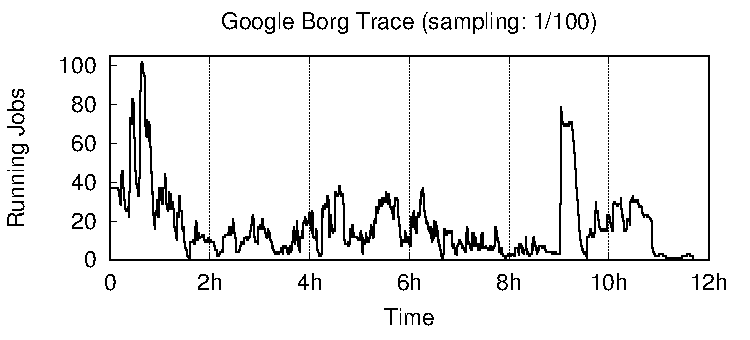
\includegraphics[]{figures/plots/borg/trace_dynamic}
  \caption{Initial 12 hours of the Google Borg Trace.}
  \label{fig:borg:dynamic}
\end{figure}

Figure~\ref{fig:borg:dynamic} shows the dynamics of the sampled workload in terms of concurrently executing jobs.
The sampled trace consists of $49,202$ jobs, with a peak of $102$ concurrent jobs, and an average job submission rate of $68.3$ jobs per minute.

For practical reasons, our experiments only consider the first $12$ hours of the trace, instead of the whole available period of 29 days.
Jobs that cross the 12-hour mark are killed abruptly.
We filter out jobs longer than $50$ minutes, as they represent less than $20\%$ of the jobs in the original trace and are not very meaningful given the 12-hour period consider.
Furthermore, in our sampling we only take into account the jobs that complete successfully.

\begin{figure}[t!]
  \centering
  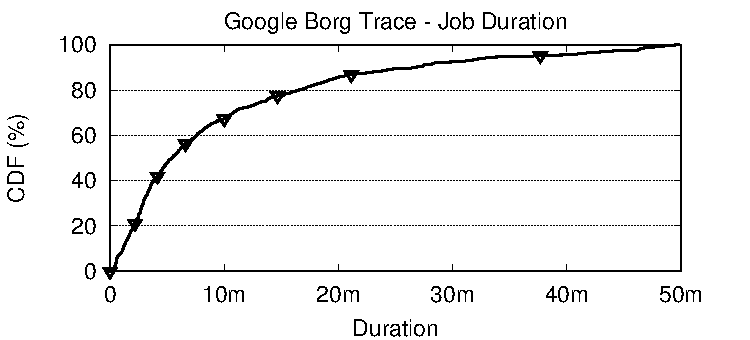
\includegraphics[]{figures/plots/borg/jobs_duration}
  \caption{Google Borg Trace: CDF of job durations.}
  \label{fig:borg:duration}
\end{figure}

Figure~\ref{fig:borg:duration} presents the duration of the jobs from the sampled trace as a \emph{cumulative distribution function} (CDF).
The considered jobs have a lifespan between $39\,s$ (the 5\emph{th} percentile) and $50\,m$ (the 100\emph{th} percentile).
Figure~\ref{fig:borg:resources} depicts the memory and CPU workload injected by the trace on our cluster.
We observe peak allocations of $42$ cores and $40\,GB$ of total memory required at any given time.

\begin{figure}[t!]
  \centering
  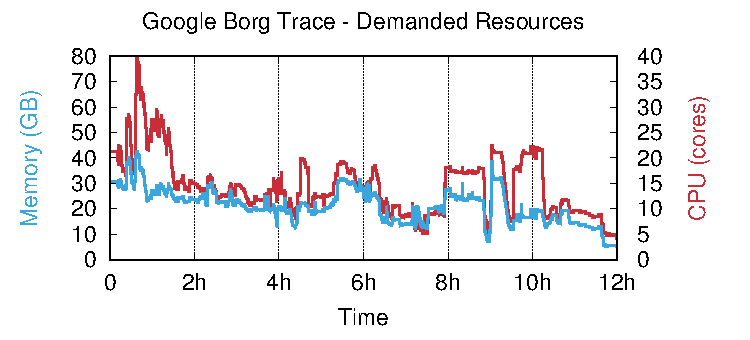
\includegraphics[]{figures/plots/borg/trace_resources}
  \caption{Google Borg Trace: demanded resources.}
  \label{fig:borg:resources}
\end{figure}

\subsection{Inside the \GP generations}
\label{subsec:eval:inside}

The \GP strategy involves the dispatch of containers and their following migration into the \emph{young} and the \emph{old} generations, according to the informations gathered during the automatic profiling phase.
Figure~\ref{fig:inside} shows the migrations occurring, during the first 2 hours, from/to the generations when \textsc{Docker Swarm} uses the \GP strategy.
We complement these results by looking at the total number of active hosts for each generation, as shown in Figure~\ref{fig:inside:generation}.
The sampled Borg trace triggers $131$ migrations from the nursery to the young and $50$ from the young to the old generation.
These results partially derive from the chosen configuration of monitoring periods.
We postpone to future work a full sensibility analysis of these parameters with respect to the Borg trace.

\begin{figure}[t!]
  \centering
  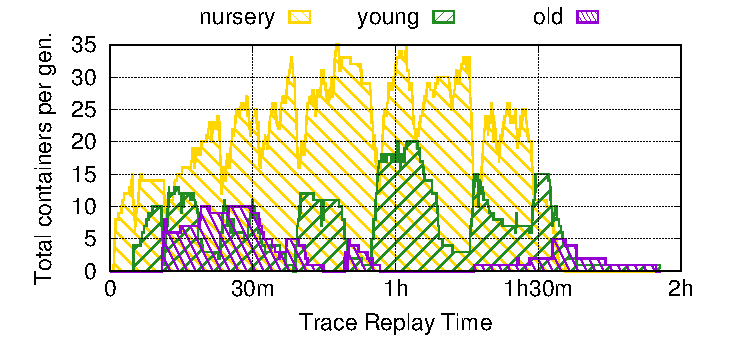
\includegraphics[]{figures/plots/containers/containers}
  \caption{Migration of containers between generations.}
  \label{fig:inside}
\end{figure}

\begin{figure}[t!]
  \centering
  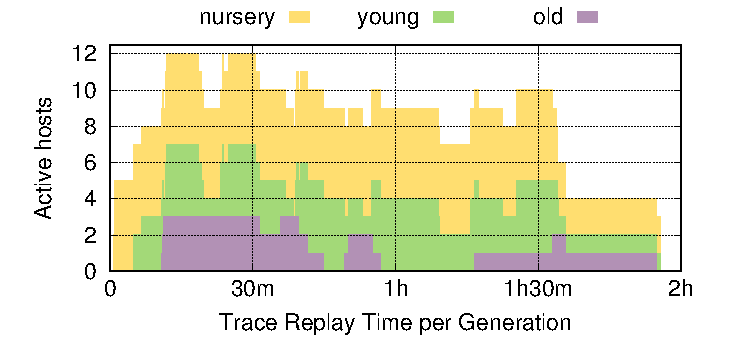
\includegraphics[]{figures/plots/containers/generation_hosts}
  \caption{Active hosts per generations.}
  \label{fig:inside:generation}
\end{figure}

While performing these experiments, we observe different replay timings---\emph{i.e.}, the time required to completely inject the Borg trace in our cluster---between the scheduling strategies under test.
Given the ideal duration of $1$ hour\vs{fix if get the results for 3 hours/12 hours/more}, the \emph{random} strategy completes in 1h19m54s, \emph{spread} in 1h02m42s, \emph{binpack} in 2h22m5s and finally the \GP strategy in 2h37m42s.
These differences can be explained by the different load on the \textsc{Docker} daemon running on the host VMs and in general the ability to load balance the containers across the hosts and VMs.
It is important to stress that these results correspond to the costs of injecting the Borg trace with our prototype, but do not directly reflect the system costs of scheduling in real conditions.
In particular, as we show in the following Section~\ref{subsec:eval:compl}, the four strategies are equivalent with respect to job completion times.


\subsection{Job completion time}
\label{subsec:eval:compl}

\begin{figure}[t!]
  \centering
  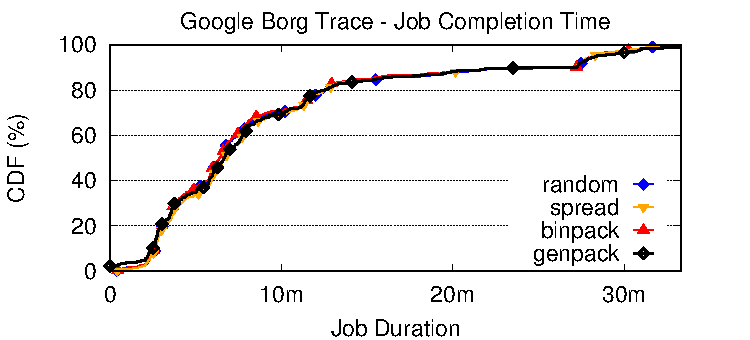
\includegraphics[]{figures/plots/completion/completion}
  \caption{Distribution (CDF) of job completion times.}
  \label{fig:completion}
\end{figure}

We compare the observed job completion time when using the default \textsc{Swarm} strategies against the \GP strategy.
Figure~\ref{fig:completion} shows that our approach does not impact negatively the executing time of the jobs.
The tested strategies result in the same long tail of few longer jobs as well as the same inflection point for the 90$^{th}$ percentile.
Instead, the $4$ strategies produce the same job completion distribution, and thus offer the same experience to the end-users of a \GP cluster.
Given the reported job completion times, we can conclude that \GP does not over-commit the cluster resources and rather offers a resource-efficient scheduling approach.

\subsection{Energy impact}
\label{subsec:eval:energy}

We demonstrate the interest of adopting the \GP strategy for a cloud data center by comparing its energy impact to the default \textsc{Swarm} strategies.
We rely on \textsc{BitWatts} probes to continuously report on the container's and node's power consumption.
Figure~\ref{fig:energy:joules} shows our results.
We present the normalized results against the \texttt{spread} baseline.
While the \texttt{binpack} strategy saves up $9\%$ of energy compared to \texttt{spread} default built-in strategy, \GP outperforms the existing strategies by saving $23\%$ of the cluster consumption.
These impressive results are due to the capability of \GP of \emph{i)} packing efficiently system containers onto a reduced number of nodes per generation and \emph{ii)} turning off unused nodes in each of the generations.
This result suggests that the \GP approach can lead to sensible savings for cloud data centers.
In particular, our evaluation based on real-world traces considers a large diversity of jobs' durations and profiles as well as incoming workloads, even though we could not inject the full Google Borg Trace.

We can also observe that the deployment of additional containers for monitoring the resource consumptions and computing the container envelopes does not penalize the power usage efficiency of \GP.
We can therefore conclude that \GP{} can achieve the same performances as existing scheduling strategies of \textsc{Docker Swarm}, but at a drastically reduced cost.

\begin{figure}[t!]
  \centering
  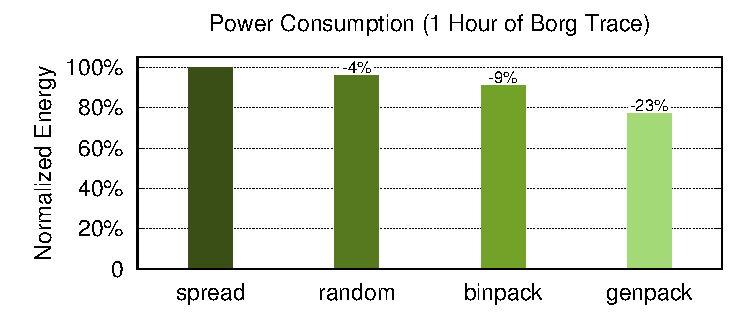
\includegraphics[]{figures/plots/energy/energy_joule}
  \caption{Normalized energy consumption.}
  \label{fig:energy:joules}
\end{figure}
